% !TEX root = ../main.tex

% Project report section

\section{Project report}


\begin{abstract}
The partial Newton sketch algorithm can be used as an approximate iterative solver for ridge regression. Following~\citet{Lacotte:2020}, we attempt to analyze the theoretical properties of partial Newton sketch for ridge regression using results from free probability and random matrix theory. We show that such an approach is not trivial and highlight the aspects of ridge regression that make doing so challenging. We make partial progress in the theory under a hypothetical trace decoupling condition and present some empirical evidence to support this hypothesis.
\end{abstract}


\subsection{Introduction}

Ridge regression is a special case of regularized least squares where the penalty function is chosen to be the $\ell_2$-norm of the model parameters. Given data matrix $\bfX\in\bbR^{n\times d}$, observations $\bfy\in\bbR^n$ and a regularization parameter $\lambda>0$, ridge regression obtains estimates of the parameters as the solution to the optimization problem
\[
\bfb^* = \argmin_{\bfb\in\bbR^d} \frac{1}{2}\|\bfX\bfb-\bfy\|_2^2 + \frac{\lambda}{2}\|\bfb\|_2^2 \;.
\]
While ridge regression can be motivated as a method for reducing overfitting in ordinary least squares (OLS), it also has its computational and analytical benefits over OLS. When $\bfX$ does not have full column rank (e.g., when $n< d$), then $\bfX^\T\bfX$ is singular and the OLS solution is non-unique. When $\bfX$ is full rank but ill-conditioned, then small changes in $\bfX$ lead to large changes in $(\bfX^\T\bfX)^{-1}$ and consequently in the OLS solution. Ridge regression addresses both of these issues by minimizing the variance and mean squared error at the cost of introducing a small bias~\citep{Chowdhury:2018}. The ridge regression solution is unique and is given by
\[
\bfb^* = \left(\bfX^\T\bfX + \lambda\bfI_d\right)^{-1}\bfX^\T\bfy \;.
\]
In this report, we analyze the theoretical properties of a partial Newton sketch algorithm~\citep{Pilanci:2017} as an iterative solver for the ridge regression problem. In particular, we attempt to derive an optimal convergence rate and an optimal step size following the approach of \citet{Lacotte:2020} for iterative Hessian sketch with OLS using asymptotic results from random matrix theory and free probability. We show that while ridge regression can be considered a simple extension to OLS, extending the analysis approach of \citet{Lacotte:2020} to partial Newton sketch is not trivial.
\\

This report is organized as follows: Section~\ref{sec:background} provides background about sketching and describes the OLS results by \citet{Lacotte:2020} that we aim to extend to ridge regression; Section~\ref{sec:literature} highlights relevant work in the literature; Section~\ref{sec:theory} discusses our attempts to analyze Newton sketch for ridge regression and the key differences from OLS that makes the problem challenging; Section~\ref{sec:empirical} describes a simulation that empirically supports one of the hypothesized theoretical conditions; and Section~\ref{sec:conclusion} summarizes our findings and concludes this report.

\subsection{Background} \label{sec:background}

This section briefly describes the Newton sketch algorithm and the probability subfields of random matrix theory and free probability that are referred to in this report.

\subsubsection{Newton's method and Newton sketch} \label{sec:newton}

Given a convex, twice-differentiable function $f:\bbR^d\rightarrow\bbR$, Newton's method is an efficient iterative method for finding the minimizing solution. The iterative updates are of the form
\[
\bfx_{t+1} = \bfx_t - \left(\nabla^2f(\bfx_t)\right)^{-1}\nabla f(\bfx_t)
\]
where $\nabla f(\bfx_t)$ and $\nabla^2f(\bfx_t)$ are the gradient and Hessian of $f$ evaluated at $\bfx_t$, respectively. Depending on the problem, computing the Hessian $\nabla^2f(\bfx_t)$ may be a computational bottleneck. The general Newton sketch algorithm~\citep{Pilanci:2017} avoids computing $\nabla^2f(\bfx_t)$ exactly and instead approximates it with
\[
\nabla^2f(\bfx_t) \approx \nabla^2f(\bfx_t)^\frac{1}{2}\bfS_t^\T\bfS_t\nabla^2f(\bfx_t)^\frac{1}{2}
\]
where $\bfS_t$ is a random, rectangular sketching matrix introduced for dimension reduction. In this project, we only consider refreshed sketches where $\bfS_0,\ldots,\bfS_t$ are \iid realizations (as opposed to a single, fixed realization) to support an analysis based on free probability. We also do not focus on the specific type of sketching matrix used as the challenges we encounter hold generally across sketch types (e.g., \iid Gaussian or orthogonal sketches).
\\

For functions with an additive decomposition of the form $f=f_0+g$, it may be sufficient for computational improvements to only do a partial Newton sketch~\citep{Pilanci:2017} where the Hessian is approximated by
\[
\nabla^2f(\bfx_t) \approx \nabla^2f_0(\bfx_t)^\frac{1}{2}\bfS_t^\T\bfS_t\nabla^2f_0(\bfx_t)^\frac{1}{2} + \nabla^2g(\bfx_t) \;.
\]
In particular, the ridge regression loss function has this form where it is analytically more convenient to consider partial Newton sketch updates.

\subsubsection{Random matrix theory and free probability} \label{sec:freeprob}

Free probability theory was initially developed by Voiculescu in the 1980's ~\citep{Anderson:2009} and is concerned with the study of non-commutative random variables. More recently, its connections to random matrix theory were established as a means of studying the limiting spectral distribution of random matrices. In free probability, the notion of freeness is analogous to independence in classical probability theory. A family of random $n\times n$ matrices $\{\bfX_n^{(1)},\ldots,\bfX_n^{(I)}\}$ is said to be asymptotically free~\citep{Couillet:2011_free} if
\begin{enumerate}
\item
$\bfX_n^{(i)}$ has a limiting spectral distribution for all $i\in\{1,\ldots,I\}$, and
\item
for all $\{i_1,\ldots,i_J\}$ with $i_j\in\{1,\ldots,I\}$, $j\in\{1,\ldots,J\}$ and $i_1\neq i_2,\ldots,i_{J-1}\neq i_J$, and for all polynomials $P_1,\ldots,P_J$ such that
\[
\lim_{n\rightarrow\infty} \frac{1}{n}\E\left[\mathrm{trace}\left(P_j\left(\bfX_n^{(i_j)}\right)\right)\right] = 0
\]
for all $j\in\{1,\ldots,J\}$, we have
\[
\lim_{n\rightarrow\infty} \frac{1}{n}\E\left[\mathrm{trace}\left(\prod_{j=1}^JP_j\left(\bfX_n^{(i_j)}\right)\right)\right] = 0 \;.
\]
\end{enumerate}
The analysis approach of \citet{Lacotte:2020} uses freeness to calculate the expected normalized trace of matrix products as for asymptotically free random matrices $\bfX_i$ and $\bfX_j$, it holds that as $n\rightarrow\infty$,
\[
\frac{1}{n}\E\left[\mathrm{trace}(\bfX_i\bfX_j)\right] - \frac{1}{n}\E\left[\mathrm{trace}(\bfX_i)\right]\frac{1}{n}\E\left[\mathrm{trace}(\bfX_j)\right] \rightarrow 0 \;.
\]
Other tools from random matrix theory such as transforms of spectral distributions are also used in their analysis, but we do not reach the stage in the analysis where they are useful in this report and so we do not cover them here.


\subsection{Related work} \label{sec:literature}

Sketched algorithms for ridge regression have been previously considered in the literature. \citet{Chowdhury:2018} examined ridge regression in the setting where $n\ll d$ and showed that under certain conditions on the sketched approximation, the relative error in the solution of the partial Newton sketch algorithm is bounded above by an exponentially decaying tolerance. \citet{Wang:2017} compared the classical sketching algorithm (i.e., sketching both the data matrix and the response vector) to the partial Newton sketch algorithm in matrix ridge regression for the case $d\ll n$ and found that both have increased risks relative to the optimal solution. They proposed model averaging as a solution for improving the theoretical properties. It is notable that the analyses by \citet{Chowdhury:2018} and \citet{Wang:2017} are both based on conventional statistical learning techniques and that the specific sketching matrix used is not a focus of the analysis.
\\

In this project, we attempt to analyze the partial Newton sketch for ridge regression following the approach that \citet{Lacotte:2020} used for iterative Hessian sketch (IHS) with OLS. Their approach relies on asymptotic results from random matrix theory and free probability, and this appeared to allow a finer-grain analysis of IHS where the derived convergence rate depends on the specific sketching matrix used. The random matrix theoretic approach to analysis does not seem to have been considered much outside of OLS problems~\citep{Dobriban:2019,Lacotte:2020b}. As we explore in this project, a possible reason for this may be that even simple extensions to standard OLS make it difficult to directly apply existing results from these subfields of probability.


\subsection{Newton sketch for ridge regression} \label{sec:ridgesketch}

Consider the ridge regression loss function
\[
f(\bfb) = \frac{1}{2}\|\bfX\bfb-\bfy\|_2^2 + \frac{\lambda}{2}\|\bfb\|_2^2
\]
for $\bfb\in\bbR^d$ given data matrix $\bfX\in\bbR^{n\times d}$ with $d\ll n$, responses $\bfy\in\bbR^n$ and a regularization parameter $\lambda>0$. The gradient and Hessian of the function are respectively given by
\begin{align*}
\nabla f(\bfb) &= \left(\bfX^\T\bfX+\lambda\bfI_d\right)\bfb - \bfX^\T\bfy \;, \\
\bfH = \nabla^2f(\bfb) &= \bfX^\T\bfX+\lambda\bfI_d \;.
\end{align*}
The Newton updates described in Section~\ref{sec:newton} therefore have the form
\begin{align*}
\bfb_{t+1} &= \bfb_t - \alpha_t\bfH^{-1}\nabla f(\bfb_t) \\
&= \bfb_t - \alpha_t\left(\bfX^\T\bfX+\lambda\bfI_d\right)^{-1}\left(\left(\bfX^\T\bfX+\lambda\bfI_d\right)\bfb_t-\bfX^\T\bfy\right) \;.
\end{align*}
A partial Newton sketch of the Hessian has the form
\[
\bfH_t = \bfX^\T\bfS_t^\T\bfS_t\bfX + \lambda\bfI_d
\]
where $\bfS_t$ is a $m\times n$ refreshed sketching matrix with $d<m\ll n$. The partial Newton sketch updates for ridge regression are then given by
\[
\bfb_{t+1} = \bfb_t - \alpha_t\left(\bfX^\T\bfS_t^\T\bfS_t\bfX + \lambda\bfI_d\right)^{-1}\left(\left(\bfX^\T\bfX+\lambda\bfI_d\right)\bfb_t-\bfX^\T\bfy\right) \;.
\]
Note that \citet{Chowdhury:2018} and \citet{Wang:2017}) also considered this sketched update for ridge regression. However, our analysis approach differs from theirs in that we adopt the asymptotic random matrix theoretic approach from \citet{Lacotte:2020}. Also note that we do not consider updates with momentum as \citet{Lacotte:2020} did as we will show that extending their analysis approach from OLS to ridge regression is already non-trivial.


\subsection{Analysis attempt based on random matrix theory} \label{sec:theory}

In this section, we show that the proof technique used to obtain Theorems~3.1 and 4.1 of \citep{Lacotte:2020} do not easily generalize to the partial Newton sketch updates for ridge regression. We follow the general procedure of the proofs and show how far we can get with the ridge regression setup. We also highlight the key differences between OLS and ridge regression that leads to problems in the proof and discuss possible solutions for rectifying these problems in future work.
\\

The following conjecture formalizes the result analogous to Theorems~3.1 and 4.1 that we would like to prove. Note that additional assumptions will be added to the conjecture as we progress through the proof.

\begin{conjecture} \label{con:ridge}
Consider the partial Newton update for ridge regression described in Section~\ref{sec:ridgesketch}. Let $\bfX = \bfU\Sigma\bfV^\T$ be the thin singular value decomposition of $\bfX$ where $\bfU$ is a $n\times d$ semi-orthogonal matrix, $\bfV$ is a $d\times d$ orthogonal matrix, and $\Sigma$ is a $d\times d$ diagonal matrix with the singular values of $\bfX$ on the diagonal. Define the error vector $\Delta_t=\bfU^\T\bfX\left(\bfb_t-\bfb^*\right)$. For some optimal step size $\alpha_t$, the sequence of error vectors $\{\Delta_t\}$ satisfies
\[
\rho = \left(\lim_{n\rightarrow\infty}\frac{\E\left[\|\Delta_t\|_2^2\right]}{\|\Delta_0\|_2^2}\right)^\frac{1}{t}
\]
where $\rho$ is the optimal rate of convergence with some closed-form expression.
\end{conjecture}

We begin our attempt to prove Conjecture~\ref{con:ridge} following the proofs by \citet{Lacotte:2020}. Using the fact that the ridge regression solution satisfies the equation
\[
(\bfX^\T\bfX + \lambda\bfI_d)\bfb^* = \bfX^\T\bfY \;,
\]
the update can be rewritten as
\begin{align*}
\bfb_{t+1} &= \bfb_t - \alpha_t\left(\bfX^\T\bfS_t^\T\bfS_t\bfX + \lambda\bfI_d\right)^{-1}\left(\left(\bfX^\T\bfX+\lambda\bfI_d\right)\bfb_t-\left(\bfX^\T\bfX+\lambda\bfI_d\right)\bfb^*\right) \\
&= \bfb_t - \alpha_t\left(\bfX^\T\bfS_t^\T\bfS_t\bfX + \lambda\bfI_d\right)^{-1}\left(\bfX^\T\bfX+\lambda\bfI_d\right)\left(\bfb_t-\bfb^*\right) \;.
\end{align*}
Using the thin SVD of $\bfX$, we have the matrix identities
\begin{align*}
\bfX^\T\bfX+\lambda\bfI_d &= \bfV\Sigma^2\bfV^\T + \lambda \bfV\bfV^\T \\
&= \bfV\left(\Sigma^2+ \lambda\bfI_d\right)\bfV^\T \;, \\
\left(\bfX^\T\bfS_t^\T\bfS_t\bfX + \lambda\bfI_d\right)^{-1} &= \left(\bfV\Sigma\bfU^\T\bfS_t^\T\bfS_t\bfU\Sigma\bfV^\T + \lambda\bfV\bfV^\T\right)^{-1} \\
&= \bfV\left(\Sigma\bfU^\T\bfS_t^\T\bfS_t\bfU\Sigma + \lambda\bfI_d\right)^{-1}\bfV^\T \;.
\end{align*}
However, in order to later on obtain an expression in terms of $\Delta_t$ as in the original proof, we require that the data matrix be full column rank. This is a less than ideal assumption to make as one of the advantages of ridge regression is being able to obtain an unique solution with non-full rank data matrices. We return to this point in Section~\ref{sec:fullrank} to discuss how this assumption may be avoided.

\begin{assumption} \label{asp:rank}
The data matrix $\bfX$ has full column rank.
\end{assumption}

Under Assumption~\ref{asp:rank}, the singular values of $\bfX$ are non-zero and so the above matrices can be rewritten as
\begin{align*}
\bfX^\T\bfX+\lambda\bfI_d &= \bfV\Sigma\left(\bfI_d + \lambda\Sigma^{-2}\right)\Sigma\bfV^\T \;, \\
\left(\bfX^\T\bfS_t^\T\bfS_t\bfX + \lambda\bfI_d\right)^{-1} &= \bfV\Sigma^{-1}\left(\bfU^\T\bfS_t^\T\bfS_t\bfU + \lambda\Sigma^{-2}\right)^{-1}\Sigma^{-1}\bfV^\T \;.
\end{align*}
Replacing the corresponding matrices in the update with these identities gives
\[
\bfb_{t+1} = \bfb_t - \alpha_t\bfV\Sigma^{-1}\left(\bfU^\T\bfS_t^\T\bfS_t\bfU + \lambda\Sigma^{-2}\right)^{-1}\left(\bfI_d + \lambda\Sigma^{-2} \right)\Sigma\bfV^\T\left(\bfb_t-\bfb^*\right) \;.
\]
Multiplying both sides by $\bfU^\T\bfX$ gives
\begin{align*}
\bfU^\T\bfX\bfb_{t+1} &= \bfU^\T\bfX\bfb_t - \alpha_t\bfU^\T\bfX\bfV\Sigma^{-1}\left(\bfU^\T\bfS_t^\T\bfS_t\bfU + \lambda\Sigma^{-2}\right)^{-1}\left(\bfI_d + \lambda\Sigma^{-2} \right)\Sigma\bfV^\T\left(\bfb_t-\bfb^*\right) \\
&= \bfU^\T\bfX\bfb_t - \alpha_t\left(\bfU^\T\bfS_t^\T\bfS_t\bfU + \lambda\Sigma^{-2}\right)^{-1}\left(\bfI_d + \lambda\Sigma^{-2} \right)\Sigma\bfV^\T\left(\bfb_t-\bfb^*\right)
\end{align*}
and then subtracting both sides by $\bfU^\T\bfX\bfb^*$ gives
\begin{align*}
\bfU^\T\bfX(\bfb_{t+1}-\bfb^*) &= \bfU^\T\bfX(\bfb_t-\bfb^*) - \alpha_t\left(\bfU^\T\bfS_t^\T\bfS_t\bfU + \lambda\Sigma^{-2}\right)^{-1}\left(\bfI_d + \lambda\Sigma^{-2} \right)\Sigma\bfV^\T\left(\bfb_t-\bfb^*\right) \\
&= \left(\bfI_d - \alpha_t\left(\bfU^\T\bfS_t^\T\bfS_t\bfU + \lambda\Sigma^{-2}\right)^{-1}\left(\bfI_d + \lambda\Sigma^{-2}\right)\right)\bfU^\T\bfX\left(\bfb_t-\bfb^*\right) \;.
\end{align*}
Let $\bfQ_t=\bfI_d - \alpha_t\left(\bfU^\T\bfS_t^\T\bfS_t\bfU + \lambda\Sigma^{-2}\right)^{-1}\left(\bfI_d + \lambda\Sigma^{-2}\right)$. Therefore by definition, we have $\Delta_{t+1} = \bfQ_t\Delta_t$ and
\[
\|\Delta_{t+1}\|^2 = \Delta_t^\T\bfQ_t^\T\bfQ_t\Delta_t \;.
\]
Taking the expectation with respect to $\bfS_t$, we get
\[
\E\left[\|\Delta_{t+1}\|^2\right] = \Delta_t^\T\E\left[\bfQ_t^\T\bfQ_t\right]\Delta_t
\]
where
\begin{align*}
\E\left[\bfQ_t^\T\bfQ_t\right] &= \bfI_d - \alpha_t\E\left[\left(\bfU^\T\bfS_t^\T\bfS_t\bfU + \lambda\Sigma^{-2}\right)^{-1}\right]\left(\bfI_d + \lambda\Sigma^{-2}\right) \\
&\quad - \alpha_t\left(\bfI_d + \lambda\Sigma^{-2}\right)\E\left[\left(\bfU^\T\bfS_t^\T\bfS_t\bfU + \lambda\Sigma^{-2}\right)^{-1}\right] \\
&\quad + \alpha_t^2\left(\bfI_d + \lambda\Sigma^{-2}\right)\E\left[\left(\bfU^\T\bfS_t^\T\bfS_t\bfU + \lambda\Sigma^{-2}\right)^{-2}\right]\left(\bfI_d + \lambda\Sigma^{-2}\right) \;.
\end{align*}
At this point, we run into our first major obstacle that prevents us from applying the key step of the proof of Theorem~3.1. In Theorem~3.1 for OLS, the expression that is obtained from taking the expectation is
\[
\E\left[\|\Delta_{t+1}\|^2\right] = \Delta_t^\T\E\left[\bfR_t^2\right]\Delta_t
\]
where
\[
\E\left[\bfR_t^2\right] = \bfI_d - 2\alpha_t\E\left[\left(\bfU^\T\bfS_t^\T\bfS_t\bfU\right)^{-1}\right] + \alpha_t^2\E\left[\left(\bfU^\T\bfS_t^\T\bfS_t\bfU\right)^{-2}\right] \;.
\]
The proof of Theorem~3.1 proceeds to recognize that the matrix $\bfS_t\bfU$ can be embedded into a Haar matrix and is therefore rotationally invariant. Using exchangeability arguments, the matrix $\E\left[\left(\bfU^\T\bfS_t^\T\bfS_t\bfU\right)^{-p}\right]$ has a simple closed-form expression in terms of the inverse moments from which the rest of the proof follows. We do not have rotational invariance in our ridge regression case, and so we follow the proof of Theorem~4.1 from this point onwards. Theorem~4.1 requires an additional assumption on the initialization of the problem in order to avoid computing the expectations directly.

\begin{assumption} \label{asp:initialization}
The initial error vector $\Delta_0$ is random, independent of $\bfS_0,\ldots,\bfS_t$, and satisfies $\E\left[\Delta_0\Delta_0^\T\right]=\frac{\bfI_d}{d}$.\footnote{The convergence rate $\rho$ in the statement of Conjecture~\ref{con:ridge} is also redefined as $\left(\lim_{n\rightarrow\infty}\frac{\E\left[\|\Delta_t\|_2^2\right]}{\E\left[\|\Delta_0\|_2^2\right]}\right)^\frac{1}{t}$ where $\E\left[\|\Delta_0\|_2^2\right]=\E\left[\Delta_0^\T\Delta_0\right]=\mathrm{trace}\left(\E\left[\Delta_0\Delta_0^\T\right]\right)=1$.}
\end{assumption}

Under Assumption~\ref{asp:initialization}, taking the expectation with respect to $\bfS_t$ gives
\begin{align*}
\E\left[\|\Delta_{t+1}\|^2\right] &= \E\left[\Delta_t^\T\bfQ_t^\T\bfQ_t\Delta_t\right] \\
&= \E\left[\Delta_0^\T\bfQ_0^\T\ldots \bfQ_t^\T\bfQ_t\ldots\bfQ_0\Delta_0\right] \\
&= \E\left[\mathrm{trace}\left(\Delta_0^\T\bfQ_0^\T\ldots \bfQ_t^\T\bfQ_t\ldots\bfQ_0\Delta_0\right)\right] \\
&= \mathrm{trace}\left(\E\left[\bfQ_0^\T\ldots \bfQ_t^\T\bfQ_t\ldots\bfQ_0\Delta_0\Delta_0^\T\right]\right) \;.
\end{align*}
By the independence of $\Delta_0$ and $\bfQ_i$, we then have
\begin{align*}
\E\left[\|\Delta_{t+1}\|^2\right] &= \mathrm{trace}\left(\E\left[\bfQ_0^\T\ldots \bfQ_t^\T\bfQ_t\ldots\bfQ_0\right]\E\left[\Delta_0\Delta_0^\T\right]\right) \\
&= \frac{1}{d}\mathrm{trace}\left(\E\left[\bfQ_1^\T\ldots \bfQ_t^\T\bfQ_t\ldots\bfQ_0\bfQ_0^\T\right]\right) \;.
\end{align*}
At this point in the proof of Theorem~4.1 for OLS, \citet{Lacotte:2020} use the asymptotic freeness of $\bfR_0\bfR_0^\T=\bfR_0^2=\left(\bfI_d-\alpha_0\bfU^\T\bfS_0^\T\bfS_0\bfU\right)^2$ and $\bfR_t\ldots\bfR_1$ to obtain a closed-form expression for the trace. Asymptotic freeness of these matrices seem to follow from Corollary~4.1 of \citep{Couillet:2011_free}, which says that for $d\times d$ Hermitian random matrices $\{\bfT_1,\ldots,\bfT_t\}$ with convergent limiting spectral distributions and Haar matrices $\{\bfW_1,\ldots,\bfW_t\}$ independent of $\bfT_i$, the random matrices $\bfW_1\bfT_1\bfW_1^\T,\ldots,\bfW_t\bfT_t\bfW_t^\T$ are asymptotically free as $n\rightarrow\infty$. Because $\bfR_0^2$ and $\bfR_i$ for $i\neq 0$ are independent and Hermitian, they each have a decomposition of the form $\bfW\bfT\bfW^\T$ where $\bfW$ is a Haar matrix and $\bfT$ is diagonal and so the result applies. However, it is less obvious that this result applies in the ridge regression case for
\begin{align*}
\bfQ_0\bfQ_0^\T &= \bfI_d - \alpha_0\left(\bfU^\T\bfS_0^\T\bfS_0\bfU + \lambda\Sigma^{-2}\right)^{-1}\left(\bfI_d + \lambda\Sigma^{-2}\right) \\
&\quad -  \alpha_0\left(\bfI_d + \lambda\Sigma^{-2}\right)\left(\bfU^\T\bfS_0^\T\bfS_0\bfU + \lambda\Sigma^{-2}\right)^{-1} \\
&\quad + \alpha_0^2\left(\bfU^\T\bfS_0^\T\bfS_0\bfU + \lambda\Sigma^{-2}\right)^{-1}\left(\bfI_d + \lambda\Sigma^{-2}\right)^2\left(\bfU^\T\bfS_0^\T\bfS_0\bfU + \lambda\Sigma^{-2}\right)^{-1}
\end{align*}
and $\bfQ_t\ldots\bfQ_1$ as individual $\bfQ_i$ and $\bfQ_i^\T$ are not Hermitian. Due to time constraints on this project, we move forward under the hypothetical assumption that asymptotic freeness is retained in the ridge regression case. \textit{If $\bfQ_0\bfQ_0^\T$ were asymptotically free from $\bfQ_t\ldots\bfQ_1$}, then from recursive application we obtain
\begin{align*}
\lim_{n\rightarrow\infty}\E\left[\|\Delta_{t+1}\|^2\right] &= \lim_{n\rightarrow\infty}\frac{1}{d}\mathrm{trace}\left(\E\left[\bfQ_2^\T\ldots \bfQ_t^\T\bfQ_t\ldots\bfQ_2\bfQ_1\bfQ_1^\T\right]\right)\lim_{n\rightarrow\infty}\frac{1}{d}\mathrm{trace}\left(\E\left[\bfQ_0\bfQ_0^\T\right]\right) \\
&= \prod_{i=0}^t\lim_{n\rightarrow\infty}\frac{1}{d}\mathrm{trace}\left(\E\left[\bfQ_i\bfQ_i^\T\right]\right) \\
&= \prod_{i=0}^t\lim_{n\rightarrow\infty}\frac{1}{d}\mathrm{trace}\left(\E\left[\bfQ_i^\T\bfQ_i\right]\right) \;.
\end{align*}
Using the expression for $\E\left[\bfQ_i^\T\bfQ_i\right]$ given earlier, we have
\begin{align*}
\lim_{n\rightarrow\infty}\frac{1}{d}\mathrm{trace}\left(\E\left[\bfQ_i^\T\bfQ_i\right]\right) &= 1 - \lim_{n\rightarrow\infty}\frac{2\alpha_i}{d}\mathrm{trace}\left(\E\left[\left(\bfU^\T\bfS_i^\T\bfS_i\bfU + \lambda\Sigma^{-2}\right)^{-1}\right]\left(\bfI_d + \lambda\Sigma^{-2}\right)\right) \\
&\quad + \lim_{n\rightarrow\infty}\frac{\alpha_i^2}{d}\mathrm{trace}\left(\E\left[\left(\bfU^\T\bfS_i^\T\bfS_i\bfU + \lambda\Sigma^{-2}\right)^{-2}\right]\left(\bfI_d + \lambda\Sigma^{-2}\right)^2\right) \;.
\end{align*}
Our final obstacle then comes from giving a closed-form expression for the limiting spectral distributions of the above matrices. The proof of Lemma~3.2 (specifically, sub-Lemma~A.1) by \citet{Lacotte:2020} that derives closed-form expressions for the inverse moments of the limiting spectral distribution of $\bfU^\T\bfS_i^\T\bfS_i\bfU$ does not work for the ridge regression case as the proof again relies on embedding $\bfS_i\bfU$ into a Haar matrix. A different approach would be necessary and we leave this for future work due to time constraints on this project.
\\

Assuming that the singular values $\sigma_i$ of $\bfX$ along with their inverses $\sigma_i^{-1}$ are bounded as $n\rightarrow\infty$, the limiting spectral distribution of $\bfQ_i$ exists when it exists for $\bfU^\T\bfS_i^\T\bfS_i\bfU$. Hypothetically, \textit{if constant closed-form expressions of the limiting traces could be derived}, then the next step would be to minimize $\lim_{n\rightarrow\infty}\E\left[\|\Delta_{t+1}\|^2\right] = \rho(\alpha)^{t+1}$ as a function of constant step size $\alpha$. Note that $\rho(\alpha)$ is quadratic and convex in $\alpha$. Furthermore, because $\bfQ_i^\T\bfQ_i$ is positive semidefinite, its trace is non-negative and therefore $\rho(\alpha)\geq0$. Thus, minimizing the limiting error norm is equivalent to minimizing $\rho(\alpha)$. Doing so leads to a step size $\alpha$ that is asymptotically optimal (under our assumptions) for a ridge regression solver with partial Newton sketch updates.


\subsubsection{Full column rank assumption} \label{sec:fullrank}

We revisit the full rank data matrix assumption (Assumption~\ref{asp:rank}) and consider the implications if it were relaxed. As mentioned, requiring the data matrix to have full column rank is not ideal for ridge regression as one possible reason for using it over OLS is to enforce an unique solution when the data matrix is not full rank. The assumption is made by \citet{Lacotte:2020} and in our analysis following theirs so that the singular values of $\bfX$ are positive and therefore $\Sigma$ is invertible. This allows for factorizing out $\Sigma$ from the matrix product containing the random matrix, and the remaining product $\bfU^\T\bfS_0^\T\bfS_0\bfU$ then has properties that \citet{Lacotte:2020} exploit. In the ridge regression case, factorizing out $\Sigma$ does not appear to lead to a particularly convenient form and so we explore the consequences of not doing so.
\\

Using the original identities
\begin{align*}
\bfX^\T\bfX+\lambda\bfI_d &= \bfV\left(\Sigma^2+ \lambda\bfI_d\right)\bfV^\T \;, \\
\left(\bfX^\T\bfS_t^\T\bfS_t\bfX + \lambda\bfI_d\right)^{-1} &= \bfV\left(\Sigma\bfU^\T\bfS_t^\T\bfS_t\bfU\Sigma + \lambda\bfI_d\right)^{-1}\bfV^\T \;,
\end{align*}
we obtain an update of the form
\[
\bfb_{t+1} = \bfb_t - \alpha_t\bfV\left(\Sigma\bfU^\T\bfS_t^\T\bfS_t\bfU\Sigma + \lambda\bfI_d\right)^{-1}\left(\Sigma^2 + \lambda\bfI_d \right)\bfV^\T\left(\bfb_t-\bfb^*\right) \;.
\]
Notice that multiplying both sides by $\bfV^\T$ gives
\[
\bfV^\T\bfb_{t+1} = \bfV^\T\bfb_t - \alpha_t\left(\Sigma\bfU^\T\bfS_t^\T\bfS_t\bfU\Sigma + \lambda\bfI_d\right)^{-1}\left(\Sigma^2 + \lambda\bfI_d \right)\bfV^\T\left(\bfb_t-\bfb^*\right)
\]
and then subtracting both sides by $\bfV^\T\bfb^*$ gives
\begin{align*}
\bfV^\T(\bfb_{t+1}-\bfb^*) &= \bfV^\T(\bfb_t-\bfb^*) - \alpha_t\left(\Sigma\bfU^\T\bfS_t^\T\bfS_t\bfU\Sigma + \lambda\bfI_d\right)^{-1}\left(\Sigma^2 + \lambda\bfI_d \right)\bfV^\T\left(\bfb_t-\bfb^*\right) \\
&= \left(\bfI_d - \alpha_t\left(\Sigma\bfU^\T\bfS_t^\T\bfS_t\bfU\Sigma + \lambda\bfI_d\right)^{-1}\left(\Sigma^2 + \lambda\bfI_d \right)\right)\bfV^\T\left(\bfb_t-\bfb^*\right) \;.
\end{align*}
This form is potentially interesting as we can initiate an analysis similar to the original approach but with the error vector instead defined as $\Delta_t=\bfV^\T(\bfb_t-\bfb^*)$, i.e., as some projection of the solution error as opposed to some projection of the prediction error. Following the steps in the original approach, under Assumption~\ref{asp:initialization}, we again arrive at
\[
\E\left[\|\Delta_{t+1}\|^2\right] = \frac{1}{d}\mathrm{trace}\left(\E\left[\bfQ_1^\T\ldots \bfQ_t^\T\bfQ_t\ldots\bfQ_0\bfQ_0^\T\right]\right)
\]
where now $\bfQ_i = \bfI_d-\alpha_i\left(\Sigma\bfU^\T\bfS_i^\T\bfS_i\bfU\Sigma + \lambda\bfI_d\right)^{-1}\left(\Sigma^2 + \lambda\bfI_d \right)$. Here, we run into the same challenges with applying results from free probability as in the first approach. While the matrix $\Sigma\bfU^\T\bfS_i^\T\bfS_i\bfU\Sigma$ may appear more complicated to work with than $\bfU^\T\bfS_i^\T\bfS_i\bfU$ in the first approach, its structure has been studied in the free probability literature. For example, Theorem~4.11 of \citep{Couillet:2011_free} says that for a matrix of the form
\[
\bfD^\frac{1}{2}\bfW\bfT\bfW^\T\bfD^\frac{1}{2}
\]
where $\bfD$ and $\bfT$ are diagonal non-negative matrives and $\bfW$ is a Haar matrix, the $\eta$-transform of the limiting spectral distribution exists and satisfies a certain set of equations. We can obtain the form specified in this result by diagonalizing $\bfS_i^\T\bfS_i$. While this particular result does not help with discerning asymptotic freeness, it does show that such matrix structure has been considered in the literature and that it may have further properties that could potentially be useful.


\subsection{Empirical experiments} \label{sec:empirical}

In Section~\ref{sec:theory}, we were unable to prove that asymptotic freeness holds for $\bfQ_1^\T\ldots\bfQ_t^\T\bfQ_t\ldots\bfQ_1$ where $\bfQ_i=\bfI_d - \alpha_i\left(\bfU^\T\bfS_i^\T\bfS_i\bfU + \lambda\Sigma^{-2}\right)^{-1}\left(\bfI_d + \lambda\Sigma^{-2}\right)$. In this section, we at least empirically investigate the trace decoupling property mentioned in Section~\ref{sec:freeprob} through a simple study where we examine the error
\[
\delta(n,\xi) = \frac{1}{d}\mathrm{trace}\left(\E\left[\bfQ_1^\T\bfQ_2^\T\bfQ_3^\T\bfQ_3\bfQ_2\bfQ_1\right]\right) - \frac{1}{d^3}\prod_{i=1}^3\mathrm{trace}\left(\E\left[\bfQ_i^\T\bfQ_i\right]\right)
\]
and how it changes as $n,d$ and $m$ grow proportionally according to fixed ratios $\gamma=\frac{d}{n}$ and $\xi=\frac{m}{n}$.
\\

We take $\gamma=0.05$ and consider two values of $\xi\in\{0.1,0.2\}$ in our study. We take $\bfX$ to be a $n\times d$ matrix of \iid standard Gaussians where $n\in\{256,512,1024,2048\}$ (corresponding to $n=2^p$ for $p\in\{8,\ldots,11\}$) and $d=\left\lceil{\gamma n}\right\rceil$. For $m=\left\lceil{\xi n}\right\rceil$, we take $\bfS_i$ to be refreshed $m\times n$ sketching matrices of one of the following types:
\begin{enumerate}
\item
\iid Gaussian: entries are \iid Gaussian random variables with mean 0 and variance $m^{-1}$.
\item
Haar: entries are generated by sampling \iid standard Gaussian random variables and then applying the Gram-Schmidt procedure to obtain a semi-orthogonal matrix.
\item
Subsampled randomized Hadamard transform (SRHT) \citep{Lacotte:2020}: the matrix $\bfS_i$ is not formed explicitly. Instead, the left singular vectors $\bfU$ of $\bfX$ are transformed through the map $\bfU\mapsto \bfB\bfH_n\bfD\bfP\bfU$ where $\bfP$ is a random permutation matrix, $\bfD$ is a diagonal matrix with Rademacher random variables on the diagonal, $\bfH_n$ is the $n\times n$ Walsh-Hadamard matrix, and $\bfB$ is a diagonal matrix with Bernoulli$\left(\frac{m}{n}\right)$ on the diagonal. The rows of the output matrix corresponding to the zero rows of $\bfB$ are discarded and so the sketch $\bfS_i\bfU$ is only approximately a $m\times n$ matrix.
\end{enumerate}
We set $\lambda=0.1$. As we were also unable to determine the optimal step sizes $\alpha_i$ in Section~\ref{sec:theory}, for convenience we use the constant step size
\[
\alpha= \frac{(\xi-\gamma)^2}{\gamma^2+\xi-2\gamma\xi}
\]
which is the optimal (asymptotic) step size for IHS with refreshed orthogonal sketches~\citep{Lacotte:2020}. This corresponds to step sizes of $\alpha\approx0.027$ for $\xi=0.1$ and $\alpha\approx0.123$ for $\xi=0.2$.
\\

Figure~\ref{fig:rmse} shows the estimated root mean squared error (RMSE) for each of the three sketch types where the squared error $\delta(n,\xi)^2$ is averaged over 50 independent simulations for each configuration of $n$ and $\xi$. In all configurations, the RMSE appears to converge to 0 as the dimensions grow which supports the trace decoupling hypothesis. For smaller $n$, the orthogonal sketches have larger RMSE compared to the \iid Gaussian sketches, though their RMSE appear to decrease more rapidly on average than that of the \iid Gaussian sketches. An interesting note is that the sketch ratio $\xi$ does not seem affect the RMSE for \iid Gaussian sketches, though a larger sketch size does significantly decrease the RMSE for orthogonal sketches.

\begin{figure}[ht]
\centering
\begin{minipage}[c]{0.21\textwidth}
\vspace{2em}
\end{minipage}
\hfill
\begin{minipage}[c]{0.76\textwidth}
\hfill $\xi=0.1$ \qquad\qquad\; \hfill $\xi=0.2$ \qquad\qquad\; \hfill
\end{minipage} \\
\begin{minipage}[c]{0.21\textwidth}
\hfill \textbf{\iid Gaussian}
\end{minipage}
\hfill
\begin{minipage}[c]{0.76\textwidth}
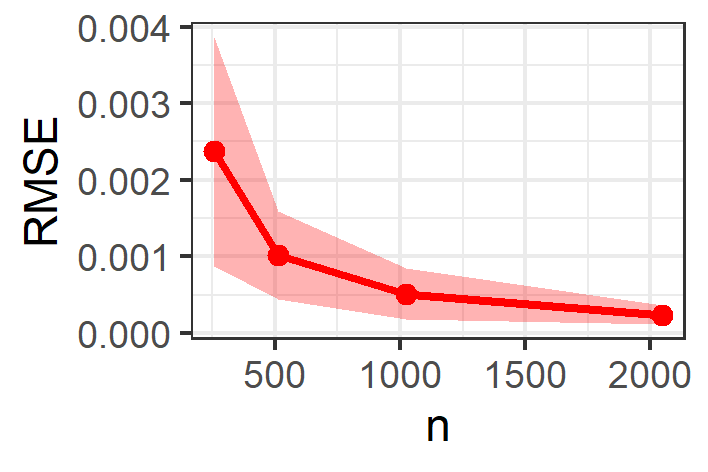
\includegraphics{images/rmse_sketchgaussian_xi0.1.png}
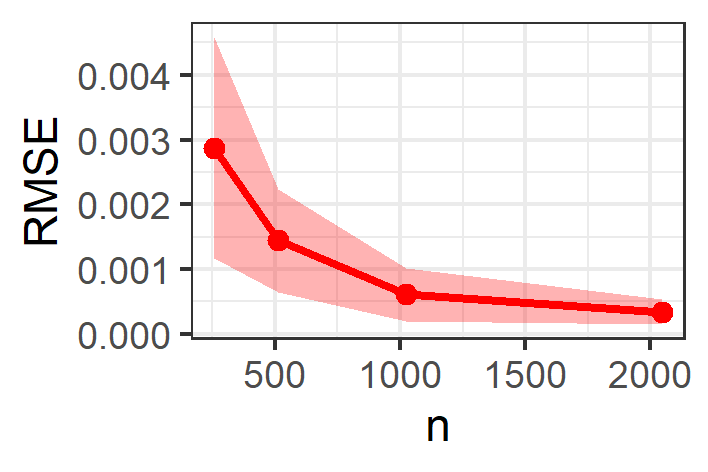
\includegraphics{images/rmse_sketchgaussian_xi0.2.png}
\end{minipage} \\
\begin{minipage}[c]{0.21\textwidth}
\hfill \textbf{Haar}
\end{minipage}
\hfill
\begin{minipage}[c]{0.76\textwidth}
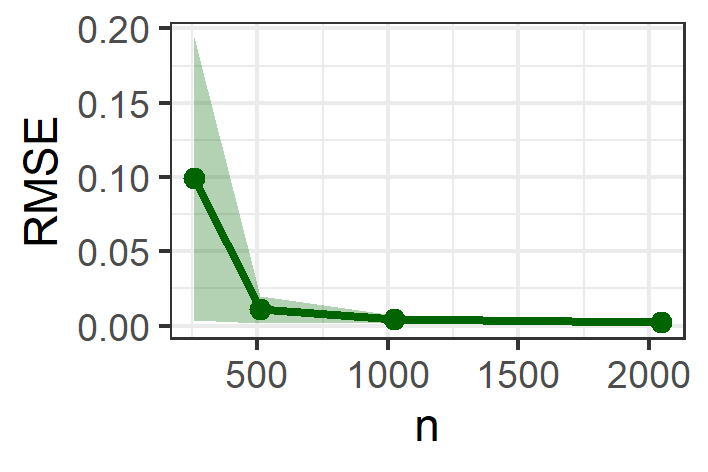
\includegraphics{images/rmse_sketchhaar_xi0.1.png}
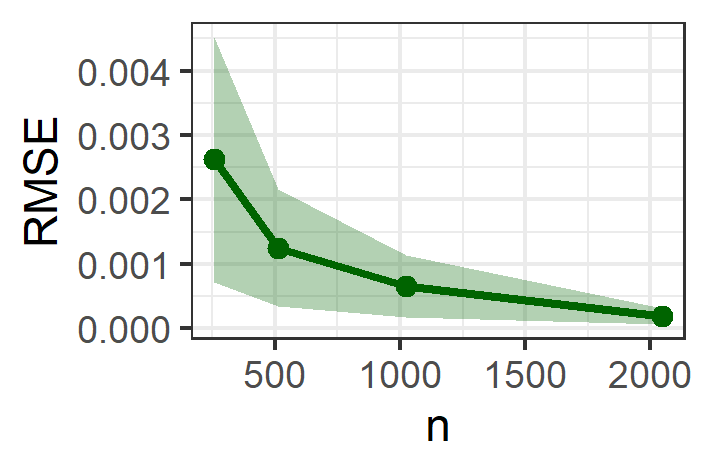
\includegraphics{images/rmse_sketchhaar_xi0.2.png}
\end{minipage} \\
\begin{minipage}[c]{0.21\textwidth}
\hfill \textbf{SRHT}
\end{minipage}
\hfill
\begin{minipage}[c]{0.76\textwidth}
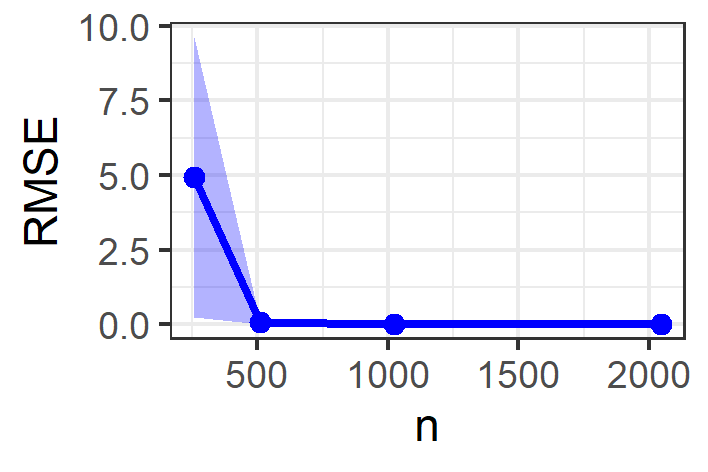
\includegraphics{images/rmse_sketchsrht_xi0.1.png}
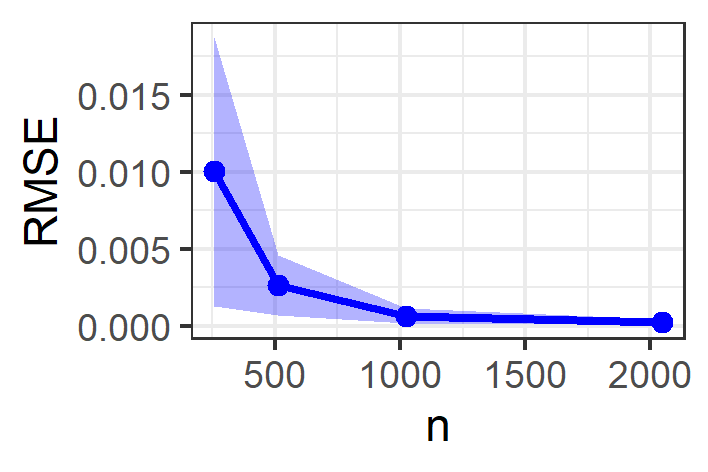
\includegraphics{images/rmse_sketchsrht_xi0.2.png}
\end{minipage}
\caption{The estimated RMSE and standard error for $\xi\in\{0.1,0.2\}$ and \iid Gaussian, Haar and SRHT sketches. The mean and standard error at each point is calculated over 50 independent simulations.}
\label{fig:rmse}
\end{figure}


\subsection{Discussion} \label{sec:conclusion}

In this project, we showed that extending the analysis of \citet{Lacotte:2020} for OLS with IHS to ridge regression with partial Newton sketch is not trivial. The main challenges in attempting to do so come from not being able to directly apply existing results from free probability and random matrix theory to the matrices obtained from the ridge regression updates that are analogous to the ones in the OLS updates. Under certain assumptions and a number of hypothetical conditions, we outlined a procedure to derive the optimal convergence rate and corresponding step size for sketched ridge regression. We examined the full column rank data matrix assumption and showed that relaxing this assumption may lead to a similar analysis but with a different criterion (in terms of the solution error). Through simulations, we empirically showed that the trace decoupling condition hypothesized in the theory appears to hold in at least one simple experimental setting. Though the simulation does not explore all parameters of potential interest (e.g., other values of $\gamma$, $\lambda$, etc.), the results do instill some optimism that the theory may hold.
\\

One thing to note is that the partial Newton sketch algorithm we considered in this project uses refreshed sketches, i.e., sketching matrices that are resampled every iteration. Results addressing the asymptotic freeness of matrices would not apply to fixed sketches due to the matrices no longer being independent, and thus an analysis based on free probability would likely be unsuitable for the fixed sketch case. Empirical results from \citet{Chowdhury:2018} do suggest that refreshed sketches enable faster convergence than fixed sketches for ridge regression (in at least one context), and so the fixed sketch case may not be particularly interesting anyways.
\\

Due to the time constraints on this project, there is much work left incomplete and a number of possible directions for future work. One direction is to complete the analysis and verify the asymptotic freeness of the matrices in the proof, as well as to determine whether closed-form expressions of the inverse moments are possible. It may also be of interest to explore whether this analysis approach can be used for other sketch-based methods, though our impression is that given the current state of the free probability and random matrix theory literature, there will only be a narrow set of methods and problems for which such an analysis may be applied. This seems to be the case as to our knowledge, there are only a handful of works~\citep{Dobriban:2019,Lacotte:2020,Lacotte:2020b} in the sketching literature that have used this analysis approach. However, free probability and random matrix theory seems to be an active area of research and so new developments may change this outlook.
